\chapter{Rule mining on extended knowledge graphs}
In this chapter, we first briefly summarize the \gls{kg} extension and mining process, before exploring each component separately.

The process starts with a \gls{kg}. From this \gls{kg}, we want to first mine rules, then extend it with new plausible facts, and lastly mine rules again on the extended \gls{kg}. Candidates for additions to the \gls{kg} are generated according to strategies that attempt to maximise the candidates’ plausibility. Once this set of candidate triples has been generated, the best of these are added to the \gls{kg}. While there is no direct way to give an absolute score to these triples, a \gls{kge} trained on the original \gls{kg} can rank the candidate triples against a set of corrupted triples. With the candidates ranked, one can accept all candidates above some appropriately chosen cutoff and add them to the \gls{kg}. Then rules can be mined and evaluated on both the original and extended \gls{kg}, and results can be compared.

\begin{figure}[htp]
    \centering
    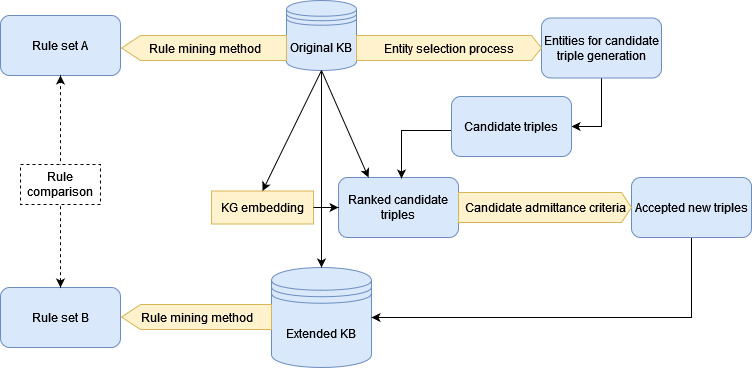
\includegraphics[width=16cm]{figures/ontology_mining_pipeline.jpg}
    \caption[Experiment pipeline diagram.]{Diagram representing \gls{kg} extension and rule mining pipeline.}
\end{figure}

This chapter also looks at the datasets used in the experiments and the results from the model selection process. The goal of the model selection process is to produce \gls{kge} models of acceptable quality for the data extension pipeline. Since the models are merely components of the process and not experimental results, this chapter presents the model selection outcomes.

\section{KG datasets}
While there are many large \glspl{kg} publicly available, they are often quite complex in the number of different relations and entities used. Since we are mining rules over relations, the range of different relations was kept small. By restricting the number of relations, the resulting rules will not be overly diverse, and there will be many more candidate triples per relation when generating new plausible triples. Two different datasets were used to conduct the experiments, both of which were limited to contain only six different types of relations. We discuss them next as we look at the \glspl{kg} individually.


\subsection{Wikidata5M-family KG}
Wikidata5M is a \gls{kg} dataset containing over 20 million triples with over 800 types of relations. It combines information from the Wikidata \gls{kg} with Wikipedia pages \cite{wang2019kepler}. Wikidata5M uses the same identifier system as Wikidata, where each entity and relation is assigned a unique integer ID. The IDs of entities are prefixed with the letter \texttt{Q} and those of relations with \texttt{P}. For example, the following line \\
\centerline{\texttt{\href{https://www.wikidata.org/wiki/Q146}{Q146} \quad \href{https://www.wikidata.org/wiki/Property:P279}{P279} \quad  \href{https://www.wikidata.org/wiki/Q39201}{Q39201}}} \
corresponds to \textless\texttt{\href{https://www.wikidata.org/wiki/Q146}{house cat}, \href{https://www.wikidata.org/wiki/Property:P279}{subclass of}, \href{https://www.wikidata.org/wiki/Q39201}{pet}}\textgreater, where each entity has a corresponding Wikipedia page.
This dataset was chosen due to its size and because it contained family-related information. Rules about family structure are well-known and easy to comprehend. For example, the simple rule $parent(a, b) \Rightarrow  child(b, a)$ would be implicitly represented in the \gls{kg}.
\begin{lstlisting}[float, language=Python, caption={Python dictionary converting family predicate IDs to their names.},captionpos=t, label={family_predicated_dict}]
family_predicates_dict = {
    'P40': 'child', 
    'P22' : 'father', 
    'P25' : 'mother',
    'P26' : 'spouse', 
    'P1038' : 'relative', 
    'P3373' : 'sibling', 
}
\end{lstlisting}

All triples that did not use one of the six selected family predicates were filtered out, and the IDs were converted to meaningful names so that the resulting rules mined would be easily readable. The python dictionary in \cref{family_predicated_dict} shows the chosen predicates. A few other family predicates were considered, but did not have enough corresponding data points or were too similar to other selected predicates. Common family-related predicates such as \texttt{grandchild} or \texttt{sister} are also not currently used in Wikidata. From a discussion in the Wikidata community, it seems that all properties considered redundant were removed \cite{kinship_discussion}. Pykeen's distribution of the dataset was used for the experiments \cite{ali2021pykeen}. The resulting subset of Wikidata5M contained around 250 000 triples and will henceforth be referred to as the \textit{family KG}.

\subsection{WN18RR}
WN18RR is a smaller \gls{kg} with 93 003 triples and only 11 relations \cite{dettmers2018convolutional}. It is an improved version of the WN18 dataset, where it was found that there was information leakage between the training and test set of WN18. Many test triples could be identified simply by inverting triples in the training set \cite{toutanova2015observed}. For example, the relation \texttt{has\_child} is the inverse relation of \texttt{has\_parent}, meaning that if the triple \texttt{(Ann, has\_parent, Carol)} is in the training set, then one can infer that \texttt{(Carol, has\_child, Ann)} likely is in the test set, thereby the test data is no longer consideres "unseen" not a fair data set to evaluate the model on. WN18RR addresses this issue.

WN18RR contains triples scraped from WordNet, a lexical database for English \cite{wordNet}. In WordNet nouns, verbs, adjectives, and adverbs are grouped into sets of semantic synonyms called
\textit{synsets} which express a distinct concept. For example, \texttt{\{man\}} and \texttt{\{adult male\}} belong to the same synset. Synsets are connected to other synsets by semantic relations. The most commonly used relation in WN18RR is \texttt{hypernym}. A synset \texttt{X} is a hypernym of synset \texttt{Y}, if every \texttt{Y} is a kind of \texttt{X}. For example, the triple 
\centerline{\texttt{02121808 \quad hypernym \quad 02121620}}
represents the information that the synset \texttt{cat} is a hypernym of the synset \texttt{house cat}. Or more simply phrased: \textit{All house cats are cats}.

\begin{table}[ht]
\centering
\begin{tabular}{|c|c|c|}
\hline
& \textbf{Relation} & \textbf{Frequency}\\
\hline
\multirow{6}{*}{\rotatebox[origin=c]{90}{Included}} &hypernym & 36873\\
&derivationally related form & 31865\\
&member meronym & 7912\\
&has part & 5131\\
&synset domain topic of & 3328\\
&instance hypernym & 3118\\
\hline
\multirow{5}{*}{\rotatebox[origin=c]{90}{Excluded}}&also see & 1396\\
&verb group & 1220\\
&member of domain region & 981\\
&member of domain usage & 673\\
&similar to & 86\\
\hline
\end{tabular}
\caption[Freq. of relations in WN18RR.]{Frequency of relations in WN18RR \gls{kg} and whether they were included in the final \gls{kg}.}
\end{table}

Though it is not vital for the reader to understand the semantics behind the relations in this dataset, it may be more rewarding to understand the terms when later reading rules mined from the WN18RR \gls{kg}. The relation \texttt{hypernym} was described above, so now the remaining five relations are succinctly explained.
\begin{itemize}
    \item \texttt{derivationally related form} \newline A concept $A$ derives from another concept $B$. \texttt{perfectly} is the derivationally related form of \texttt{perfect}.
    \item \texttt{member meronym}  \newline A concept $A$ is a member of a concept $B$. \texttt{class} is a member meronym of \texttt{student}.
    \item \texttt{has part} \newline A whole concept $A$ has a part $B$. \texttt{cat} has part \texttt{tail}.
    \item \texttt{synset domain topic of}  \newline A concept $A$ is the scientific field which concept $B$ belongs in. \texttt{computer science} is the synset domain topic of \texttt{deep learning}.
    \item \texttt{instance hypernym}  \newline It denotes the type of an instance. For example, \texttt{Bergen} has instance hypernym \texttt{city}.
\end{itemize}

WN18RR was chosen due to the few number of relations in it, and with a \gls{kg} already containing few relations, most of the data could be included.
By taking all triples containing one of the six most frequent relations, in total 88227 datapoints, 95\% of WN18RR was used. This was intended to produce a more complete \gls{kg}. The dataset was loaded using AmpliGraph \cite{ampligraph}.

\section{KGE model architectures}
\label{selected_KG_embedding_models}
There are many publicly available knowledge graph embedding libraries \cite{libkge, chandrahas-etal-2018-towards, ali2021pykeen}. The library AmpliGraph was chosen due to its thorough documentation and because it is an open source library based on Tensorflow, a well-known library for the development of machine learning models \cite{tensorflow}. The library provides many different \gls{kge} models, performance metrics, and \gls{kg} datasets. Three different \gls{kge} methods were selected: TransE, DistMult, and ComplEx. 

TransE was selected because it is one of the simplest and most intuitive \gls{kge} models. Due to the limited number of relations in the \glspl{kg}, this architecture may be sufficient for producing a good embedding. However, as mentioned in section \ref{KG_embeddings_section}, TransE struggles with learning complex and symmetric relations, both of which are present in the chosen \glspl{kg}, therefore it may not be adequate. In the family \gls{kg} \textit{spouse} and \textit{relative} are symmetric relationships. \textit{child} is an example of a complex relation, as a person can have many children. In WN18RR \textit{derivationally related form} is symmetric, but not reflexive.

DistMult was selected because it is in a different family of embedding vectors, namely tensor-factorization based models. Recalling its description from section \ref{KG_embeddings_section}, DistMult is one of the least computationally-intensive models due to its use of diagonal matrices, which made it an obvious choice for the experiments of this thesis.

ComplEx has the same runtime as DistMult, and was therefore an attractive candidate. The embedding model was chosen due to this and also because it addresses DistMult's shortcomings in embedding antisymmetric relations. The relations \textit{parent} and \textit{child} in the family \gls{kg} are antisymmetric, so it would be interesting to compare the results from these two models.

AmpliGraph also provides a baseline model, to which the three selected models were compared to. The baseline model, called RandomBaseline, assigns a pseudo-random score to each triples it is asked to evaluate. When it comes to extending the \gls{kg} this would essentially have the same effect as adding noise to the data.

\section{Model selection}
Each \gls{kge} model has a number of hyperparameters that can be optimised. As the search space grows, it has been shown that random search is more optimal than grid search, where each combination needs to be tested \cite{bergstra2012random}. Due to limited computational resources, this approach to hyperparameter optimisation was selected. It is not an optimal approach, but serves as a practical and effective solution that measures well against more sophisticated methods such as Baysian optimisation \cite{li2017hyperband}.

\begin{table}[htbp]
\centering
\begin{tabular}{l|l}
\textbf{Hyperparameter}      & \textbf{Values}             \\ \hline
Batches count       & 50, 100                              \\ 
Epocs               & 50, 100                          \\ 
Embedding dimension                   & 50, 100, 200                     \\ 
$\eta$ (negative sampes @ rate)     & 5, 10, 15                            \\ 
Loss function   & pairwise, nll                         \\ 
Pairwise loss margin    & 0.5, 1, 2                    
%Regularizer         & LP                             \\ \hline
%Learning rate       & Random number in range(0.0001, 0.01) \\ \hline
\end{tabular}
%\label{{hyperparameter_table}
\caption[Hyperparameter values for model selection.]{Hyperparameter values to search through during model selection.}
\end{table}

\begin{table}[htbp]
\centering
\begin{tabular}{l|ccc|ccc}
\multicolumn{1}{c|}{\multirow{2}{*}{\textbf{PARAM.}}} & \multicolumn{3}{c|}{\textbf{WN18RR}}                                                                                  & \multicolumn{3}{c}{\textbf{Family}}                                                                                  \\ \cline{2-7} 
\multicolumn{1}{c|}{}                                 & \multicolumn{1}{c|}{\textbf{TransE}} & \multicolumn{1}{c|}{\textbf{DistMult}} & \multicolumn{1}{c|}{\textbf{ComplEx}} & \multicolumn{1}{c|}{\textbf{TransE}} & \multicolumn{1}{c|}{\textbf{DistMult}} & \multicolumn{1}{c}{\textbf{ComplEx}} \\ \hline
\textbf{Batch size}                                 & 50                                   & 50                                     & 100                                   & 50                                   & 100                                    & 50                                    \\
\textbf{Epocs}                                         & 50                                   & 100                                    & 100                                   & 50                                   & 50                                     & 100                                   \\
\textbf{Emb. dim.}                                     & 50                                   & 200                                    & 100                                   & 50                                   & 200                                    & 200                                   \\
\textbf{$\eta$}                           & 15                                   & 5                                      & 10                                    & 15                                   & 10                                     & 15                                    \\
\textbf{Loss func.}                                 & nll                                  & nll                                    & pairwise                              & nll                                  & nll                                    & nll                                   \\
\textbf{P. l. margin}                                & -                                    & -                                      & 0.5                                   & -                                    & -                                      & -                                    
\end{tabular}
\caption[Hyperparameter selection results]{Hyperparameter selection results. The hyperparameter at the bottom of the table, pairwise loss margin, was only applicable for those models that used a pairwise loss function, hence the missing values.}
\label{hyperparameter_selection_results}
\end{table}


The AmpliGraph documentation was the primary inspiration when deciding which hyperparameters to focus on. It was, for example, stated in the documentation that they received the best results with the adam optimizer, therefore other optimisers were not considered in the hyperparameter search \cite{ampligraph_documentation}. For each hyperparameter combination, a learning rate randomly chosen in the range of 0.0001 - 0.01 was selected, yet another design choice borrowed from AmpliGraph.

For the implementation of model selection, AmpliGraph's \texttt{select\_best\_mode\_ranking} was used. It is a model selection routine that allows for both grid and random search. At the end of each model selection process, the final model for each embedding type is retrained on the concatenation of the train and validation set, before it is eventually evaluated on the test set. The \texttt{eta} hyperparameter denotes the number of negative examples generated at training for each positive example, a process described in section \ref{KG_embeddings}. The hyperparameters for the final selected models can be seen in table \ref{hyperparameter_selection_results}. % As the training data only contains positive examples, negative ones are generated.  In the training process corrupted triples are generated according to the strategy proposed by Bordes et al, which maintains the local closed world assumption \cite{TransE}.

\subsection{Model selection results}
The final model of all three embedding architectures had good results on the WN18RR dataset, and even better results on the family \gls{kg}. Each model had an \gls{mrr} score above 0.9 on the family \gls{kg} and around 0.6 on the WN18RR. TransE seemed to perform slightly worse than DistMult and ComplEx on the family \gls{kg}. On the WN18RR dataset TransE had a lower hits@1 score, while it outperformed both DistMult and ComplEx in both hits@3 and hits@10.
\begin{table}[htbp]
\centering
\begin{tabular}{l||ccccc||ccccc}

{\textbf{DATASET}}                 & \multicolumn{5}{c||}{\textbf{WN18RR}}                                                                                                                                               & \multicolumn{5}{c}{\textbf{Family KG}}                                                                                                                            \\ \hline
\multirow{2}{*}{{\textbf{METRIC}}} & \multicolumn{1}{c|}{\multirow{2}{*}{\textbf{MR}}} & \multicolumn{1}{c|}{\multirow{2}{*}{\textbf{MRR}}} & \multicolumn{3}{c||}{\textbf{Hits@}}                                       & \multicolumn{1}{c|}{\multirow{2}{*}{\textbf{MR}}} & \multicolumn{1}{c|}{\multirow{2}{*}{\textbf{MRR}}} & \multicolumn{3}{c}{\textbf{Hits@}}                                       \\ \cline{4-6} \cline{9-11} 
                                       & \multicolumn{1}{c|}{}                             & \multicolumn{1}{c|}{}                              & \multicolumn{1}{l|}{\textbf{1}} & \multicolumn{1}{l|}{\textbf{3}} & \multicolumn{1}{l||}{\textbf{10}} & \multicolumn{1}{c|}{}                             & \multicolumn{1}{c|}{}                              & \multicolumn{1}{l|}{\textbf{1}} & \multicolumn{1}{l|}{\textbf{3}} & \multicolumn{1}{l}{\textbf{10}} \\ \hline
\textbf{Baseline}       & 495.32     & 0.007      & 0     & 0       & 0.01        & 498.72       & 0     & 0       & 0       & 0.1      \\ 
\textbf{TransE}  & 34.29  & 0.60       & 0.51                     & 0.66    & 0.76 & 2.59     & 0.93  &0.88  & 0.97   & 0.99   \\ 
\textbf{DistMult}      & 152.37  & 0.62    & 0.59   & 0.63      & 0.66   & 7.45    & 0.98     & 0.98    & 0.99   & 0.99    \\ 
\textbf{ComplEx}        & 139.36    & 0.59      & 0.57      & 0.60      & 0.63      & 4.64     & 0.99     & 0.98     & 0.99      & 0.99  
\end{tabular}
\caption[Test results of selected model.]{Results of selected models evaluated on test set.}
\end{table}


\begin{figure}[htbp]
\centering
\begin{subfigure}{.5\textwidth}
  \centering
  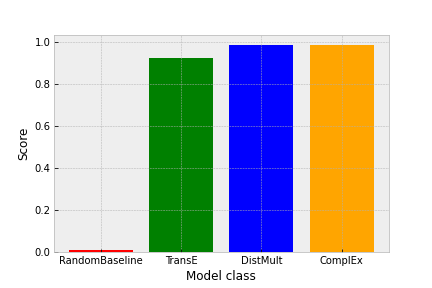
\includegraphics[width=1\linewidth]{figures/model_selection/family_mrr.png}
  \caption{\gls{mrr} scores}
  \label{fig:model_selection_mrr_family}
\end{subfigure}%
\begin{subfigure}{.5\textwidth}
  \centering
  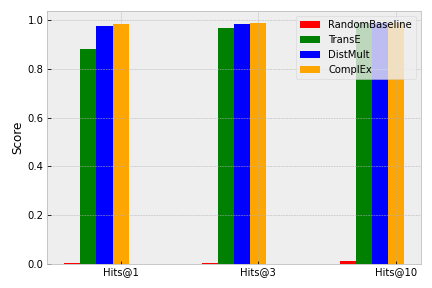
\includegraphics[width=1\linewidth]{figures/model_selection/family_hit_scores.png}
  \caption{Hits@k scores}
  \label{fig:model_selection_hit_scores_family}
\end{subfigure}
\caption[KGE test results for family KG.]{\gls{kge} test performance results for family \gls{kg}.}
\label{fig:model_selection_metrics_family}
\end{figure}

\begin{figure}[htbp]
\centering
\begin{subfigure}{.5\textwidth}
  \centering
  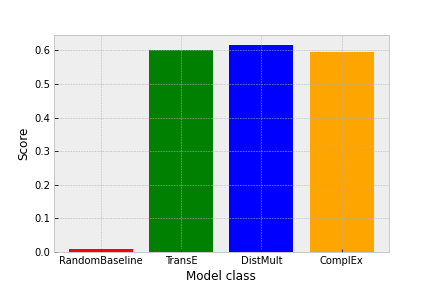
\includegraphics[width=1\linewidth]{figures/model_selection/wn18rr_mrr.png}
  \caption{\gls{mrr} scores}
  \label{fig:model_selection_mrr_wn18rr}
\end{subfigure}%
\begin{subfigure}{.5\textwidth}
  \centering
  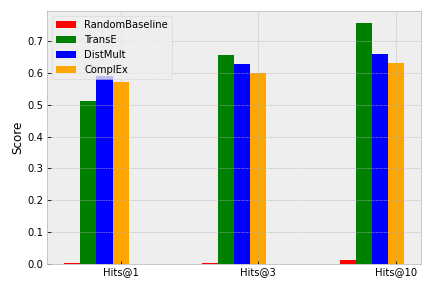
\includegraphics[width=1\linewidth]{figures/model_selection/wn18rr_hit_scores.png}
  \caption{Hits@k scores}
  \label{fig:model_selection_hit_scores_wn18rr}
\end{subfigure}
\caption[KGE test results for WN18RR KG.]{\gls{kge} test performance results for WN18RR.}
\label{fig:model_selection_metrics_wn18rr}
\end{figure}



%epochs (int) – The iterations of the training loop.

%batches_count (int) – The number of batches in which the training set must be split during the training loop.

%k (int) – Embedding space dimensionality.

%loss : pairwise loss, with a margin of 0.5 set via the loss_params kwarg.

\newpage

\section{KG extension}

The goal of \gls{kg} extension is to add potentially true statements to the original \gls{kg}. AmpliGraph does have an implementation for this, called \texttt{discover\_facts}, but due to computational limitations\footnote{\texttt{discover\_facts} uses \textit{all} entities in the \gls{kg} to generate counterexamples. In large \glspl{kg} like the ones used in our experiments, this is not feasible.} it could not be used.
However, the implementation used in our study follows the same general strategy used in \texttt{discover\_facts}. It consists of two main components:
\begin{enumerate}
    \item Candidate triple generation
    \item Ranking of generated candidates
\end{enumerate}
With a set of ranked candidate triples, all that remains is to decide the minimum rank for a candidate to be admitted to the \gls{kg}.


\subsection{Candidate triple generation}
\label{canidate_triple_generation}
Both in the family \gls{kg} and in WN18RR the number of potential facts is enormous, and so in order to avoid having to evaluate all of them, several strategies can be used to select plausible facts. In AmpliGraph's implementation of plausible candidate generation, they make the assumption that densely connected entities are less likely to have missing true statements. In a \gls{kge} tutorial at the European Conference on Artificial Intelligence in 2020, members of the AmpliGraph team claim that this assumption has been true for their empirical evaluations, but is not necessarily true for all datasets \cite{kge_tutorial}.  As stated, AmpliGraph has implemented different strategies, many of which have to do with graph clustering, but these were too computationally intensive to be used. Four simpler strategies for entity selection were instead used:
\begin{itemize}
    \item Random selection of entities.
    \item Selecting the most frequent entities.
    \item Selecting the least frequent entities.
    \item Probabilistic selection based on the frequency of the entities in the dataset, where the least frequent entities are most likely to be selected.
\end{itemize}

\begin{table}[htbp]
\centering
\begin{tabular}{rcl|lcc}
\multicolumn{3}{c|}{\textbf{KG}}                    &  & \multicolumn{1}{l}{\textbf{Entity}} & \multicolumn{1}{l}{\textbf{Freq.}} \\\hline
\textit{Ann} & \textit{sibling} & \textit{Bob}   &  & Ann                               & 4                                      \\
\textit{Ann} & \textit{sibling} & \textit{Carl} &  & Bob                                 & 3                                      \\
\textit{Ann} & \textit{friend}  & \textit{Carl} &  & Carl                               & 3                                      \\
\textit{Bob}   & \textit{friend}  & \textit{Carl} &  & Dave                                & 2                                      \\
\textit{Bob}   & \textit{friend}  & \textit{Dave}  &  & Eve                                 & 2                                      \\
\textit{Ann} & \textit{friend}  & \textit{Eve}   &  & Felix                               & 1                                      \\
\textit{Felix} & \textit{friend}  & \textit{Gina}  &  & Gina                                & 1                                      \\
\textit{Dave}  & \textit{friend}  & \textit{Eve}   &  & \multicolumn{1}{l}{}                & \multicolumn{1}{l}{}                  
\end{tabular}
\caption[Example KG with frequency table of entities.]{Example \gls{kg} with frequency table of entities.}
\label{entity_selection_KG}
\end{table}

If we look at listing \ref{entity_selection_KG} as an example \gls{kg} and need to select three entities for candidate generate, then with the 
\begin{itemize}
    \item \textit{most frequent} strategy the entity set would be \{\textit{Ann, Bob, Carl}\},
    \item \textit{least frequent} strategy the entity set would be \{\textit{Dave, Felix, Gina}\},
    \item \textit{probabilistic} strategy the entity set could be \{\textit{Gina, Eve, Felix}\},
\end{itemize}
and any three candidates would be selected with the \textit{random} strategy. Note that selection is without replacement. Once the entities were selected, all possible triples were generated with them and the six relations. Then, all the triples already included in the original \gls{kg} were excluded from the resulting candidate triples. If one were to pick the \textit{most frequent} strategy, then the resulting set of candidate triples would be that depicted in \cref{canidate_triples_most_frequent}. Of course, the more candidate triples there are to choose from, the better the extension will be because then there is a higher chance of plausible facts being suggested. Again, computational limitations restricted this. After trying different candidate set sizes, it was eventually decided that selecting 1000 entities for candidate triple generation was a feasible number. This meant that $ 1000 \times 6 \times 1000 = 6 \times 10^6 $ triples (minus those that already appeared in the \gls{kg}) were considered for each \gls{kg} extension.


\begin{table}[htbp]
\centering
\begin{tabular}{rcllrcl}
\multicolumn{7}{c}{\textbf{Candiate Triples}}                                                                                                                                                                                                       \\
\textit{Ann}                        & \textit{sibling}                        & \textit{Ann}                        &  & \textit{Ann}                        & \textit{friend}                        & \textit{Ann}                        \\
{\color[HTML]{CB0000} \textit{Ann}} & {\color[HTML]{CB0000} \textit{sibling}} & {\color[HTML]{CB0000} \textit{Bob}}   &  & \textit{Ann}                        & \textit{friend}                        & \textit{Bob}                          \\
{\color[HTML]{CB0000} \textit{Ann}} & {\color[HTML]{CB0000} \textit{sibling}} & {\color[HTML]{CB0000} \textit{Carl}} &  & {\color[HTML]{CB0000} \textit{Ann}} & {\color[HTML]{CB0000} \textit{friend}} & {\color[HTML]{CB0000} \textit{Carl}} \\
\textit{Bob}                          & \textit{sibling}                        & \textit{Ann}                        &  & \textit{Bob}                          & \textit{friend}                        & \textit{Ann}                        \\
\textit{Bob}                          & \textit{sibling}                        & \textit{Bob}                          &  & \textit{Bob}                          & \textit{friend}                        & \textit{Bob}                          \\
\textit{Bob}                          & \textit{sibling}                        & \textit{Carl}                        &  & {\color[HTML]{CB0000} \textit{Bob}}   & {\color[HTML]{CB0000} \textit{friend}} & {\color[HTML]{CB0000} \textit{Carl}} \\
\textit{Carl}                        & \textit{sibling}                        & \textit{Ann}                        &  & \textit{Carl}                        & \textit{friend}                        & \textit{Ann}                        \\
\textit{Carl}                        & \textit{sibling}                        & \textit{Bob}                          &  & \textit{Carl}                        & \textit{friend}                        & \textit{Bob}                          \\
\textit{Carl}                        & \textit{sibling}                        & \textit{Carl}                        &  & \textit{Carl}                        & \textit{friend}                        & \textit{Carl}                       
\end{tabular}
\caption[Candidate triples for example KG]{Candidate triples for the \gls{kg} in listing \ref{entity_selection_KG}, using entity selection method \textit{most frequent}, and entity set size 3. Triples in red are already present in the \gls{kg} and are removed from the candidates set.}
\label{canidate_triples_most_frequent}
\end{table}


\subsection{Candidate triple ranking}
As discussed in Section \ref{Performance_indicators}, it is not easy to set an absolute score to a triple with a \gls{kge}. Therefore candidate triples are instead ranked against corrupted triples. An accurate \gls{kge} model will rank well-suited candidates higher than the corrupted triples. Since only one side of each triple is corrupted at a time, the corrupted triples generated are compliant with the local closed world assumption. AmpliGraph's function \texttt{evaluate\_performance} evaluates the performance of a trained \gls{kge} model by ranking a set of test triples from the \gls{kg} against a set of corrupted triples. An embedding model is then evaluated based on how good it is at ranking the positive test triples higher than the negative corrupted triples. By instead passing the set of candidate triples to \texttt{evaluate\_performance}, these could be ranked instead. Once the candidates have been given ranks, one simply needs to decide on a cutoff rank to consider the candidate as a true fact and add it to the \gls{kg}. The rank cutoffs that were considered were 1, 4, and 7. These values were chosen as they are in the range of typical Hits@K cutoff values. Rank cutoff 1 is the strictest cutoff possible where only candidates ranked higher than \textit{all} the corrupted triples are admitted. Hits@1 is also the strictest Hit ratio performance metric, where the triple with the highest score must be a true fact in the \gls{kg}. As stated in Section \ref{Hits@k}, hit ratio cutoff values larger than 10 are rarely used. Therefore the other two rank cutoff values chosen for experiments were within this range.

\section{Rule mining and evaluation}
Rules are mined using the rule mining algorithm AMIE3 \cite{amie3}. The authors of AMIE3 have made an implementation of it available on \hyperlink{https://github.com/lajus/amie}{GitHub}. It is released as an executable jar file that takes a \gls{kg} in TSV file format as input and outputs rules accompanied by various confidence scores. The jar file in release 3.0 was used for rule mining. It was run using the default settings used in the AMIE3 paper by Lajus et al. \cite{amie3}. Since default settings change, the exact command used for rule mining was: \texttt{java -jar amie-milestone-intKB.jar -bias lazy -full -noHeuristics -ostd [TSV file]}.

As previously mentioned, the implementation of AMIE3 outputs the rules accompanied by confidence scores. Unfortunately, the scores are calculated on the same dataset the rules have been mined from. Since these datasets have been extended, they may contain datapoints that are false positives, leading to evaluation based on erroneous data. New rules that follow this incorrect data will therefore possibly receive high scores despite not making sense in the given context. To amend this problem, all mined rules are also evaluated on the original \gls{kg}.
% Jørn: Is the following paragraph relevant? no.
This was not previously available in any release of AMIE3, which only allows rule evaluation in combination with rule mining, on the dataset from which the rules are being mined. Evaluation of rules on a custom \gls{kg} was not possible until one of the authors, Jonathan Lajus, was kind enough to add a script to do exactly this.

In the final results from the experiments run, each mined rule had two different sets of confidence scores, one evaluated on the original \gls{kg} and the other on the extended \gls{kg}. In addition to scores, each rule was also accompanied by the parameters under which the \gls{kg} was extended. These three parameters are the \textit{entity selection method}, the \textit{\gls{kge} model} used to rank candidates, and the \textit{rank cutoff value} for candidate admittance. In summary, the output data points in the rule mining and evaluation process had these features:
\begin{itemize}
    \item Rule
    \item Metrics
        \subitem Head Coverage (extended and original \gls{kg})
        \subitem \gls{pca} Confidence (extended and original \gls{kg})
        \subitem Positive Examples (extended and original \gls{kg})
        \subitem \gls{pca} body size (extended and original \gls{kg})
    \item Parameters
        \subitem Entity seleciton method
        \subitem \gls{kge} model
        \subitem Rank cutoff
    \item Boolean indication for whether the rule was also mined from the original \gls{kg}
\end{itemize}

With this information, one can look at the effect the parameters have on the number of rules mined and how the measured confidence differs when calculated on the extended \gls{kg} versus the original \gls{kg}.


\section{Additional experimental setup details}
The experiments were run on a server with 64 GB of RAM and an Intel Core i9-7900X 3.3GHz processor.

The implementation of AMIE used in our study is distributed under the \hyperlink{https://creativecommons.org/licenses/by-nc/3.0/}{Creative Commons Attribution-NonComercial license v3.0} by the \hyperlink{https://www.mpi-inf.mpg.de/departments/databases-and-information-systems/research/yago-naga/amie/}{YAGO-NAGA team} and the \hyperlink{https://dig.telecom-paris.fr/blog/}{DIG team}. The program uses Javatools, a library released under the \hyperlink{https://creativecommons.org/licenses/by/3.0/}{Creative Commons Attribution license v3.0} by the \hyperlink{https://www.mpi-inf.mpg.de/departments/databases-and-information-systems/research/yago-naga/amie/}{YAGO-NAGA team}.
